\hypertarget{section}{%
\section{1 Section}\label{section}}

\hypertarget{earlier-subsection}{%
\subsection{1.1 Earlier Subsection}\label{earlier-subsection}}

\begin{figure}
\hypertarget{fig:img1}{%
\centering
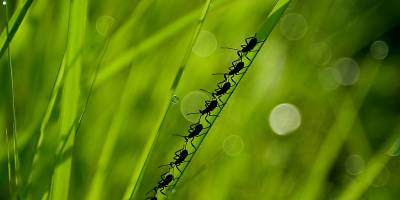
\includegraphics{img2.png}
\caption{Image 1}\label{fig:img1}
}
\end{figure}

\hypertarget{title-of-subsection}{%
\subsection{1.6 Title of Subsection}\label{title-of-subsection}}

\begin{figure}
\hypertarget{fig:img2}{%
\centering
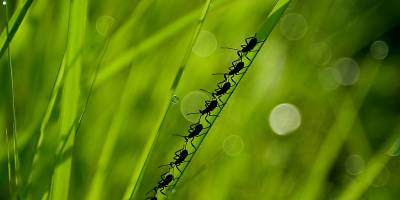
\includegraphics{img2.png}
\caption{Image 1.6.2}\label{fig:img2}
}
\end{figure}

\begin{figure}
\hypertarget{fig:img3}{%
\centering
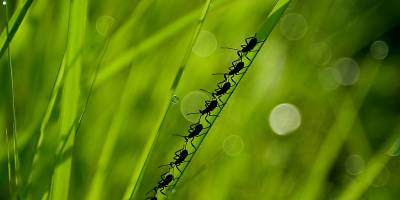
\includegraphics{img2.png}
\caption{Image 1.6.100500}\label{fig:img3}
}
\end{figure}

\begin{figure}
\hypertarget{fig:img4}{%
\centering
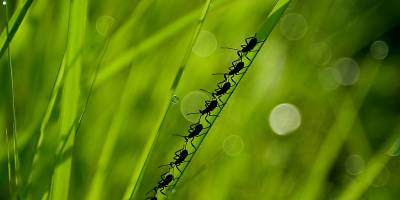
\includegraphics{img2.png}
\caption{Image 1.6.100501}\label{fig:img4}
}
\end{figure}

\hypertarget{title-of-subsection-1}{%
\subsection{1.7 Title of Subsection}\label{title-of-subsection-1}}

\begin{figure}
\hypertarget{fig:img21}{%
\centering
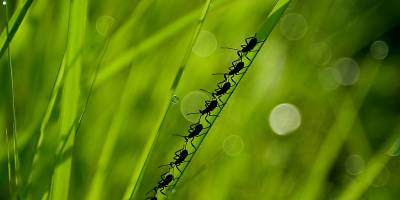
\includegraphics{img2.png}
\caption{Image 1.7.1}\label{fig:img21}
}
\end{figure}

\begin{figure}
\hypertarget{fig:img31}{%
\centering
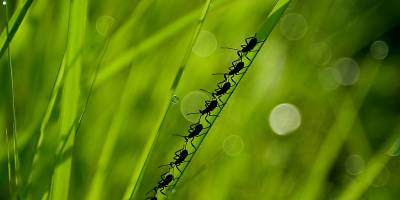
\includegraphics{img2.png}
\caption{Image 1.7.100500}\label{fig:img31}
}
\end{figure}

\begin{figure}
\hypertarget{fig:img41}{%
\centering
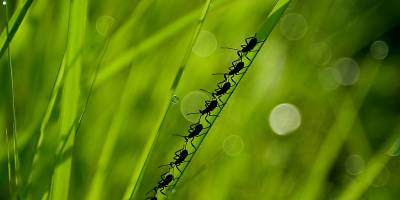
\includegraphics{img2.png}
\caption{Image 1.7.100501}\label{fig:img41}
}
\end{figure}
